%!TEX root = ../thesis.tex

\chapter{Marco Metodológico}  %Title of the First Chapter
\label{capitulo3}

\ifpdf
    \graphicspath{{metodologia/Figs/Raster/}{metodologia/Figs/PDF/}{metodologia/Figs/}}
\else
    \graphicspath{{metodologia/Figs/Vector/}{metodologia/Figs/}}
\fi

A fin de mejorar la productividad en el desarrollo y la calidad del motor de juego, se hace uso de la metodología de desarrollo por prototipos. Esta  metodología se caracteriza por la construcción de un prototipo, el cual es evaluado y usado en un ciclo de retroalimentación, en donde se refinan los requisitos del software que se desarrollará \cite{mcconnell2004code}. Esta metodología permite probar la eficacia de diferentes algoritmos y la forma que debería tomar la interacción humano-máquina a través de diferentes prototipos, aspectos importantes para este proyecto, debido a que los algoritmos tradicionales para motores de juegos diseñados para lenguajes iterativos no son ideales para su uso en lenguajes funcionales.

\begin{figure}[!htbp!]
\centering
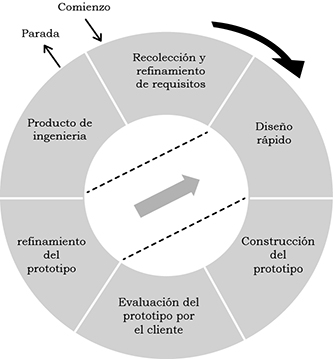
\includegraphics[width=0.5\textwidth]{metoPrototipo}
\caption[Metodología de desarrollo por prototipos]{Ciclo de desarrollo de una aplicación mediante la metodología de desarrollo por prototipos.}
\end{figure}

\section{Requisitos del sistema}

Ya que el objetivo de este proyecto es la creación de un motor de juego, los requisitos ideales que este debe suplir son los mismos que cualquier otro motor de juego, tener un motor gráfico para dibujar en pantalla, permitir a los programadores implementar la lógica de sus juegos, permitir a los artistas importar recursos al juego, un motor de física que resuelva colisiones entre objetos, entre otras características comunes antes mencionadas.

La diferencia que este proyecto debe necesariamente suplir, es funcionar en un lenguaje funcional, permitiendo a los programadores de los juegos trabajar con el mismo, y hacer el mayor uso posible de los beneficios que brinda la programación funcional para hacer que los juegos producidos sean lo más eficientes posible.

\section{Limitaciones del sistema}

Ya que crear un motor de juego con todas las características que poseen los motores profesionales es una labor colosal, este proyecto limitara las funcionalidades del programa final en lo mínimo requerido para poder producir juegos funcionales.

Las capacidades mínimas elegidas para poder producir juegos son, tener un  motor gráfico, poder cargar recursos para el motor gráfico, en este caso imágenes, shaders y mallados poligonales, y finalmente el motor lógico donde el programador implementará la funcionalidad del juego. Están serán tomadas como los requerimientos  mínimos que el programa final deberá de proveer como motor de juego, y serán usados como guía para la producción de los prototipos durante el desarrollo.

\section{Especificación de requisitos}

El programa final tendrá como usuario tres tipos de actores, que son los artistas, interesados principalmente en poder usar sus creaciones dentro del juego, los programadores, que implementan la lógica del juego usando el motor, y los jugadores, que si bien no interactúan directamente con el motor, lo hacen indirectamente a través de los juegos creados.

El principal caso de uso de los jugadores con el motor es el uso de los juegos, en ese aspecto el motor debe de encargarse de generar juego que transmitan correctamente las intenciones del jugador al sistema del juego. Para este proyecto este caso de uso se limitara a la entrada que el jugador genere vía el teclado, el ratón o modificaciones que este realice a la ventana del juego.

En cuanto a los artistas, el motor solo requiere tener la capacidad de cargar recursos para el motor gráfico.

El actor de mayor importancia para el programa final será el programador, este debe de tener la capacidad de implementar la lógica de su juego usando programación funcional, de preferencia con funciones puras. También se requerirá de un sistema que le permita correr funciones de E/S cuando se le sea necesario sin interferir con el flujo de cómputo de la lógica del juego, de preferencia en forma asíncrona. Finalmente el programador deberá de tener una manera de recibir y hacer cálculos con la entrada recibida del usuario y usar los recursos provistos por los artistas para dibujar en pantalla.

Adicionalmente de cubrir las necesidades de los actores, se espera que el motor haga el mayor uso posible de las facilidades ofrecidas por la programación funcional para hacer los que los juegos creados puedan hacer el mayor uso de los recursos del ordenador, especialmente en temas de paralelismo donde destaca la programación funcional.

\section{Arquitectura}

Los diferentes requerimientos del proyecto serán implementados en forma modular, para permitir que nuevos prototipos solo requieran la modificación de una sección del programa. Como el lenguaje de implementación \emph{Haskell} posee estándares para la construcción de paquetes y librerías \cite{wiki:WriteAHaskellProgram}, estos se utilizaran para la construcción del programa.

\section{Desarrollo}

Usando la metodología de desarrollo por prototipos, se implementará módulos que busquen satisfacer los requisitos del sistema junto con prototipos que hagan uso de estos módulos. A través de estos prototipos se decidirá la satisfacción de los requisitos y se entrará en un ciclo de corrección y ajuste.

\section{Documentación}

El presente documento servirá como el principal manual para el funcionamiento interno del programa. Para documentación que indique el uso y funcionamiento de las funciones públicas implementadas por el motor, se usara el estándar de comentarios de \emph{Haskell} para generar documentación con el programa Haddock.
